\documentclass[12pt]{article}%
%%%%%%%%%%%%%%%%%%%%%%%%%%%%%%%%%%%%%%%%%%%%%%%%%%%%%%%%%%%%%%%%%   
% All style files are available from 
%   http://wwww.uiuc.edu/~sariel/research/latex/
%%%%%%%%%%%%%%%%%%%%%%%%%%%%%%%%%%%%%%%%%%%%%%%%%%%%%%%%%%%%%%%%%%   


%%%%%%%%%%%%%%%%%%%%%%%%%%%%%%%%%%%%%%%%%%%%%%%%%%%%%%%%%%%%%%%%%%   
% Conditional compilation depending on whether this is my computer or
% not.
\IfFileExists{sariel_computer.sty}{\def\sarielComp{1}}{}
\ifx\sarielComp\undefined%
\newcommand{\SarielComp}[1]{}
\newcommand{\NotSarielComp}[1]{#1}%
\else
\newcommand{\SarielComp}[1]{#1}%
\newcommand{\NotSarielComp}[1]{}%
\fi
\newcommand{\IfPrinterVer}[2]{#2}%

%%%%%%%%%%%%%%%%%%%%%%%%%%%%%%%%%%%%%%%%%%%%%%%%%%%%%%%%%%%%%%%%%% 


\usepackage[cm]{fullpage}%
\usepackage{amsmath}%
\usepackage{amssymb}%
\usepackage[cmyk]{xcolor}%
%\usepackage{xcolor}%

\SarielComp{\usepackage{sariel_colors}}%

\usepackage[amsmath,thmmarks]{ntheorem}%
\theoremseparator{.}%

\usepackage{titlesec}%
\titlelabel{\thetitle. }%

\usepackage{graphicx}%
\usepackage{xcolor}%
\usepackage{mleftright}%
\usepackage{xspace}%
\usepackage{hyperref}%

\usepackage{caption}%

\newcommand{\hrefb}[3][black]{\href{#2}{\color{#1}{#3}}}%

\IfPrinterVer{%
   \usepackage{hyperref}%
}{%
   \usepackage{hyperref}%
   \hypersetup{%
      breaklinks,%
      ocgcolorlinks, colorlinks=true,%
      urlcolor=[rgb]{0.25,0.0,0.0},%
      linkcolor=[rgb]{0.5,0.0,0.0},%
      citecolor=[rgb]{0,0.2,0.445},%
      filecolor=[rgb]{0,0,0.4},
      anchorcolor=[rgb]={0.0,0.1,0.2}%
   }
   % \usepackage{cleveref}
}

% ----------------------------------------------------------------------
% ----------------------------------------------------------------------
% Defining theorem like environments
% ----------------------------------------------------------------------
% ----------------------------------------------------------------------
\theoremseparator{.}%

\theoremstyle{plain}%
\newtheorem{theorem}{Theorem}[section]

\newtheorem{lemma}[theorem]{Lemma}
\newtheorem{conjecture}[theorem]{Conjecture}
\newtheorem{corollary}[theorem]{Corollary}
\newtheorem{claim}[theorem]{Claim}%
\newtheorem{fact}[theorem]{Fact}
\newtheorem{observation}[theorem]{Observation}
\newtheorem{invariant}[theorem]{Invariant}
\newtheorem{question}[theorem]{Question}
\newtheorem{proposition}[theorem]{Proposition}
\newtheorem{prop}[theorem]{Proposition}
\newtheorem{openproblem}[theorem]{Open Problem}

\theoremstyle{plain}%
\theoremheaderfont{\sf} \theorembodyfont{\upshape}%
\newtheorem*{remark:unnumbered}[theorem]{Remark}%
\newtheorem*{remarks}[theorem]{Remarks}%
\newtheorem{remark}[theorem]{Remark}%
\newtheorem{definition}[theorem]{Definition}
\newtheorem{defn}[theorem]{Definition}
\newtheorem{example}[theorem]{Example}
\newtheorem{exercise}[theorem]{Exercise}
\newtheorem{problem}[theorem]{Problem}
\newtheorem{xca}[theorem]{Exercise}
\newtheorem{exercise_h}[theorem]{Exercise}
\newtheorem{assumption}[theorem]{Assumption}%

% Proof environment
\newcommand{\myqedsymbol}{\rule{2mm}{2mm}}

\theoremheaderfont{\em}%
\theorembodyfont{\upshape}%
\theoremstyle{nonumberplain}%
\theoremseparator{}%
\theoremsymbol{\myqedsymbol}%
\newtheorem{proof}{Proof:}%

\newtheorem{proofof}{Proof of\!}%

% theorem block end
%%%%%%%%%%%%%%%%%%%%%%%%%%%%%%%%%%%%%%%%%%%%%%%%%%%%%%%%%%%%%%%%%%%%


%%%%%%%%%%%%%%%%%%%%%%%%%%%%%%%%%%%%%%%%%%%%%%%%%%%%%%%%%%%%%%%%%% 5
% Color emph
\providecommand{\emphind}[1]{\emph{#1}\index{#1}}
\definecolor{nalmostblack}{rgb}{0, 0, 0.7}
\providecommand{\emphic}[2]{%
   \textcolor{nalmostblack}{%
      \textbf{\emph{#1}}}%
   \index{#2}}


\providecommand{\emphi}[1]{\emphic{#1}{#1}}

\definecolor{almostblack}{rgb}{0, 0, 0.5}
\providecommand{\emphw}[1]{{\emph{{\textcolor{almostblack}{#1}}}}}%

\providecommand{\emphOnly}[1]{\emph{\textcolor{almostblack}{\textbf{#1}}}}
% Color emph - end 
%%%%%%%%%%%%%%%%%%%%%%%%%%%%%%%%%%%%%%%%%%%%%%%%%%%%%%%%%%%%%%%%%% 5


\numberwithin{figure}{section}%
\numberwithin{table}{section}%
\numberwithin{equation}{section}%


%%%%%%%%%%%%%%%%%%%%%%%%%%%%%%%%%%%%%%%%%%%%%%%%%%%%%%%%%%%%%%%%%%%
% Sariel's thanks
%%%%%%%%%%%%%%%%%%%%%%%%%%%%%%%%%%%%%%%%%%%%%%%%%%%%%%%%%%%%%%%%%%% 

\providecommand{\tildegen}{{\protect\raisebox{-0.1cm}
      {\symbol{'176}\hspace{-0.01cm}}}}
\newcommand{\atgen}{\symbol{'100}}
\newcommand{\SarielThanks}[1]{\thanks{Department of Computer Science;
      University of Illinois; 201 N. Goodwin Avenue; Urbana, IL,
      61801, USA; {\tt sariel\atgen{}illinois.edu}; {\tt
         \url{http://sarielhp.org/}.} #1}}


%%%%%%%%%%%%%%%%%%%%%%%%%%%%%%%%%%%%%%%%%%%%%%%%%%%%%%%%%%%%%%%%%%%%%%
%    Handling references
%%%%%%%%%%%%%%%%%%%%%%%%%%%%%%%%%%%%%%%%%%%%%%%%%%%%%%%%%%%%%%%%%%%%%%

\newcommand{\HLink}[2]{\hyperref[#2]{#1~\ref*{#2}}}
\newcommand{\HLinkSuffix}[3]{\hyperref[#2]{#1\ref*{#2}{#3}}}

\newcommand{\figlab}[1]{\label{fig:#1}}
\newcommand{\figref}[1]{\HLink{Figure}{fig:#1}}

\newcommand{\thmlab}[1]{{\label{theo:#1}}}
\newcommand{\thmref}[1]{\HLink{Theorem}{theo:#1}}

\newcommand{\corlab}[1]{\label{cor:#1}}
\newcommand{\corref}[1]{\HLink{Corollary}{cor:#1}}%

\providecommand{\deflab}[1]{\label{def:#1}}
\newcommand{\defref}[1]{\HLink{Definition}{def:#1}}


\newcommand{\clmlab}[1]{\label{claim:#1}}
\newcommand{\clmref}[1]{\HLink{Claim}{claim:#1}}

\newcommand{\apndlab}[1]{\label{apnd:#1}}
\newcommand{\apndref}[1]{\HLink{Appendix}{apnd:#1}}

\newcommand{\seclab}[1]{\label{sec:#1}}
\newcommand{\secref}[1]{\HLink{Section}{sec:#1}}
\newcommand{\rectA}{\Mh{B}}%
\newcommand{\rectB}{\Mh{D}}%
\newcommand{\clientsY}[2]{\Mh{\mathsf{C}}\pth{#1,#2}}

\newcommand{\DW}{\times}
\newcommand{\ConeSet}{\Mh{\mathcal{C}}}%
\newcommand{\shrinkDY}[2]{#1_{\boxminus #2}}
\newcommand{\Rects}{\Mh{\mathcal{R}}}%


\newcommand{\itemlab}[1]{\label{item:#1}}
\newcommand{\itemref}[1]{\HLinkSuffix{}{item:#1}{}}

\newcommand{\lemlab}[1]{\label{lemma:#1}}
\newcommand{\lemref}[1]{\HLink{Lemma}{lemma:#1}}%

\providecommand{\eqlab}[1]{}%
\renewcommand{\eqlab}[1]{\label{equation:#1}}
\newcommand{\Eqref}[1]{\HLinkSuffix{Eq.~(}{equation:#1}{)}}

%%%%%%%%%%%%%%%%%%%%%%%%%%%%%%%%%%%%%%%%%%%%%%%%%%%%%%%%%%%%%%%%%%% 
% Sariel's standard commands...
%%%%%%%%%%%%%%%%%%%%%%%%%%%%%%%%%%%%%%%%%%%%%%%%%%%%%%%%%%%%%%%%%%% 

\newcommand{\remove}[1]{}%
\newcommand{\Set}[2]{\left\{ #1 \;\middle\vert\; #2 \right\}}
\newcommand{\pth}[2][\!]{\mleft({#2}\mright)}%
\newcommand{\pbrcx}[1]{\left[ {#1} \right]}%
\newcommand{\Prob}[1]{\mathop{\mathbf{Pr}}\!\pbrcx{#1}}
\newcommand{\Ex}[2][\!]{\mathop{\mathbf{E}}#1\pbrcx{#2}}

\newcommand{\ceil}[1]{\left\lceil {#1} \right\rceil}
\newcommand{\floor}[1]{\left\lfloor {#1} \right\rfloor}

\newcommand{\brc}[1]{\left\{ {#1} \right\}}
\newcommand{\cardin}[1]{\left| {#1} \right|}%

\renewcommand{\th}{th\xspace}
\newcommand{\ds}{\displaystyle}%

\renewcommand{\Re}{\mathbb{R}}%
\newcommand{\reals}{\Re}%


%%%%%%%%%%%%%%%%%%%%%%%%%%%%%%%%%%%%%%%%%%%%%%%%%%%%%%%%%%%%%%%%%%%%%%%%%
% Defining comptenum environment using enumitem
\usepackage[inline]{enumitem}

\newlist{compactenumA}{enumerate}{5}%
\setlist[compactenumA]{topsep=0pt,itemsep=-1ex,partopsep=1ex,parsep=1ex,%
   label=(\Alph*)}%

\newlist{compactenuma}{enumerate}{5}%
\setlist[compactenuma]{topsep=0pt,itemsep=-1ex,partopsep=1ex,parsep=1ex,%
   label=(\alph*)}%

\newlist{compactenumI}{enumerate}{5}%
\setlist[compactenumI]{topsep=0pt,itemsep=-1ex,partopsep=1ex,parsep=1ex,%
   label=(\Roman*)}%

\newlist{compactenumi}{enumerate}{5}%
\setlist[compactenumi]{topsep=0pt,itemsep=-1ex,partopsep=1ex,parsep=1ex,%
   label=(\roman*)}%

\newlist{compactitem}{itemize}{5}%
\setlist[compactitem]{label=\ensuremath{\bullet}}%
\setlist[compactitem]{topsep=0pt,itemsep=-1ex,partopsep=1ex,parsep=1ex,%
   label=\ensuremath{\bullet}}%


\usepackage{stmaryrd}%
\providecommand{\IntRange}[1]{\mleft\llbracket #1 \mright\rrbracket}
\newcommand{\IRX}[1]{\IntRange{#1}}%
\newcommand{\IRY}[2]{\left\llbracket #1:#2 \right\rrbracket}

%%%%%%%%%%%%%%%%%%%%%%%%%%%%%%%%%%%%%%%%%%%%%%%%%%%%%%%%%%%%%%%%%%%%%%%%%%

\usepackage{wasysym}

\newcommand{\disk}{\Mh{\ocircle}}
\newcommand{\diskVY}[2]{\disk_{\downarrow}^{#1}\pth{#2}}%




%%%%%%%%%%%%%%%%%%%%%%%%%%%%%%%%%%%%%%%%%%%%%%%%%%%%%%%%%%%%%%%%%%% 
%%%%%%%%%%%%%%%%%%%%%%%%%%%%%%%%%%%%%%%%%%%%%%%%%%%%%%%%%%%%%%%%%%% 
% Papers specific commands...
%%%%%%%%%%%%%%%%%%%%%%%%%%%%%%%%%%%%%%%%%%%%%%%%%%%%%%%%
%%%%%%%%%%%%%%%%%%%%%%%%%%%%%%%%%%%%%%%%%%%%%%%%%%%%%%%%

\providecommand{\Mh}[1]{#1}%

\newcommand{\eps}{\varepsilon}

\newcommand{\CC}{\Mh{\mathcal{C}}}%
\newcommand{\FF}{\Mh{\mathcal{F}}}%
\newcommand{\LL}{\mathcal{L}}
\newcommand{\DT}{\Mh{\mathcal{D}}}%
\newcommand{\DTX}[1]{\Mh{\mathcal{DT}}\pth{#1}}
\newcommand{\DG}{\mathcal{DG}}

\newcommand{\etal}{\textit{et~al.}\xspace}

\newcommand{\Term}[1]{\textsf{#1}}
\newcommand{\TermI}[1]{\Term{#1}\index{#1@\Term{#1}}}

\newcommand{\QSPD}{\Term{QSPD}\xspace}

\newcommand{\StavThanks}[1]{%
   \thanks{Department of Computer Science;
      University of Illinois; 201 N. Goodwin Avenue; Urbana, IL,
      61801, USA; {\tt stava2\atgen{}illinois.edu}; {\tt
         \url{https://publish.illinois.edu/stav-ashur}.} #1}}

\newcommand{\pa}{\Mh{p}}%
\newcommand{\pb}{\Mh{q}}%
\newcommand{\pc}{\Mh{u}}%
\newcommand{\pd}{\Mh{v}}%

\newcommand{\px}{\Mh{x}}%
\newcommand{\py}{\Mh{y}}%
\newcommand{\pz}{\Mh{z}}%

\newcommand{\dGY}[2]{\Mh{\mathsf{d}}\pth{#1,#2}}%
\newcommand{\dGZ}[3]{\Mh{\mathsf{d}_{#1}}\pth{#2,#3}}%
\newcommand{\dY}[2]{\left\| #1 - #2 \right\|}%


\newcommand{\dsZ}[3]{\Mh{\mathsf{d}}_{#1}\pth{#2, #3}}%
\newcommand{\dZ}[3]{\left\| #2 - #3 \right\|_{#1}}%

\newcommand{\dsY}[2]{\mathsf{d}\pth{#1,#2}}
\newcommand{\DistSetY}[2]{\dsY{#1}{#2}}%

\newcommand{\body}{\Mh{C}}%

\newcommand{\grid}{\Mh{\mathsf{K}}}%

\providecommand{\G}{\Mh{G}}%
\renewcommand{\G}{\Mh{G}}%

\newcommand{\GA}{\Mh{H}}%

\providecommand{\GB}{\Mh{I}}%
\renewcommand{\GB}{\Mh{I}}%


\newcommand{\PS}{\Mh{P}}%
\newcommand{\PSup}{\Mh{P}_\uparrow}%
\newcommand{\PSdown}{\Mh{P}_\downarrow}%

\newcommand{\QS}{\Mh{\mathcal{Q}}}%
\newcommand{\liftX}[1]{\mathrm{lift}\pth{#1}}%

\newcommand{\rect}{\Mh{R}}%

\newcommand{\EG}{\Mh{E}}%
\newcommand{\EGX}[1]{\Mh{E}\pth{#1}}%
\newcommand{\region}{\Mh{\mathcalb{r}}}%
\newcommand{\gminus}{-}%
\newcommand{\interiorX}[1]{\mathrm{int}\pth{#1}}%
\newcommand{\restrictY}[2]{#1 \cap {#2}}

\newcommand{\cpX}[1]{\Mh{\mathrm{c{}p}}\pth{#1}}%
\newcommand{\diamX}[1]{\mathrm{diam}\pth{#1}}%

\newcommand{\spread}{\Mh{\Phi}}
\newcommand{\spreadX}[1]{\spread\pth{#1}}

\newcommand{\WS}{\Mh{\mathcal{W}}}%
\newcommand{\WeightX}[1]{\Mh{\omega} \pth{#1}}
\newcommand{\diameterX}[1]{\mathrm{d{}i{}am}\pth{#1}}

\newcommand{\SSPD}{\Term{SSPD}\xspace}%

\newcommand{\PSB}{\Mh{B}}%
\newcommand{\PSC}{\Mh{C}}%

\newcommand{\PSX}{\Mh{X}}%
\newcommand{\PSY}{\Mh{Y}}%

\newcommand{\WSPD}{\Term{WSPD}\xspace}%

\newcommand{\coneY}[2]{\mathrm{cone}\pth{#1,#2}}%
\newcommand{\IS}{\Mh{\mathcal{I}}}%
\newcommand{\epsA}{\Mh{\vartheta}}%

\newcommand{\GY}[2]{\Mh{\mathcal{G}}\pth{#1, #2}}%
\newcommand{\cen}{\Mh{c}}%
\newcommand{\Pair}{\Mh{\Xi}}%

\newcommand{\XSays}[2]{{ {$\rule[-0.12cm]{0.2in}{0.5cm}$\fbox{\tt #1:}
      } #2 \marginpar{\textcolor{red}{#1}}
      {$\rule[0.1cm]{0.3in}{0.1cm}$\fbox{\tt
            end}$\rule[0.1cm]{0.3in}{0.1cm}$} } }
\newcommand{\sariel}[1]{{\XSays{Sariel}{#1}}}
\newcommand{\Sariel}[1]{{\XSays{Sariel}{#1}}}

\newcommand{\QSup}{\QS_{\uparrow}}
\newcommand{\QSdown}{\QS_{\downarrow}}


%%%%%%%%%%%%%%%%%%%%%%%%%%%%%%%%%%%%%%%%%%%%%%%%%%%%%%%%%%%%%%%%%%
%%%%%%%%%%%%%%%%%%%%%%%%%%%%%%%%%%%%%%%%%%%%%%%%%%%%%%%%%%%%%%%%%%
%%%%%%%%%%%%%%%%%%%%%%%%%%%%%%%%%%%%%%%%%%%%%%%%%%%%%%%%%%%%%%%%%%
% Restating lemmas/theorems...
%
% Example
%---------------------------------------------------------------------
% \SaveContent{\LemmaNumVerticesDepthBody}{ BLA BLA }
% 
% \begin{lemma}[{{\normalfont Proof in \apndref{num:v:depth}}}]
%       \lemlab{num:vertices:depth}%
%       \LemmaNumVerticesDepthBody{}
% \end{lemma}
%...
% \bigskip%
% \RestatementOf{\lemref{num:vertices:depth}}{\LemmaNumVerticesDepthBody}
%---------------------------------------------------------------------

\newcommand{\SaveContent}[2]{%
   \expandafter\newcommand{#1}{#2}%
}

\newcommand{\RestatementOf}[2]{
   \noindent%
   \textbf{Restatement of #1.}
   % 
   {\em #2{}}%
}

%%% End
%%%%%%%%%%%%%%%%%%%%%%%%%%%%%%%%%%%%%%%%%%%%%%%%%%%%%%%%%%%%%%%%%%
%%%%%%%%%%%%%%%%%%%%%%%%%%%%%%%%%%%%%%%%%%%%%%%%%%%%%%%%%%%%%%%%%%


%%%%%%%%%%%%%%%%%%%%%%%%%%%%%%%%%%%%%%%%%%%%%%%%%%%%%%%%%%%%%%%%%%%%%%%%
%%%%%%%%%%%%%%%%%%%%%%%%%%%%%%%%%%%%%%%%%%%%%%%%%%%%%%%%%%%%%%%%%%%%%%%%
% \mathcalb - a different font that looks a bit like mathcal

\DeclareFontFamily{U}{BOONDOX-calo}{\skewchar\font=45 }
\DeclareFontShape{U}{BOONDOX-calo}{m}{n}{<-> s*[1.05] BOONDOX-r-calo}{}
\DeclareFontShape{U}{BOONDOX-calo}{b}{n}{<-> s*[1.05] BOONDOX-b-calo}{}
\DeclareMathAlphabet{\mathcalb}{U}{BOONDOX-calo}{m}{n}
\SetMathAlphabet{\mathcalb}{bold}{U}{BOONDOX-calo}{b}{n}
\DeclareMathAlphabet{\mathbcalb}{U}{BOONDOX-calo}{b}{n}

% \mathcalb - end of file
%%%%%%%%%%%%%%%%%%%%%%%%%%%%%%%%%%%%%%%%%%%%%%%%%%%%%%%%%%%%%%%%
%%%%%%%%%%%%%%%%%%%%%%%%%%%%%%%%%%%%%%%%%%%%%%%%%%%%%%%%%%%%%%%%

\newcommand{\CHX}[1]{\mathsf{ch}\pth{#1}}%

\newcommand{\rinX}[1]{\Mh{r}_{\mathrm{in}}\pth{#1}}%
\newcommand{\routX}[1]{\Mh{R}_{\mathrm{out}}\pth{#1}}%
\newcommand{\arX}[1]{\Mh{\mathsf{a{}r}}\pth{#1}}%
\newcommand{\Elp}{\Mh{\mathcal{E}}}

\newcommand{\cell}{\Mh{\mathsf{C}}}%

\newcommand{\Of}{\Mh{\mathcal{O}}}%
\newcommand{\Oeps}{\Mh{\mathcal{O}_\eps}}%
\newcommand{\gConst}{\Mh{\tau}}%
\newcommand{\xSlabX}[1]{\overleftrightarrow{#1}}
\newcommand{\ySlabX}[1]{\updownarrow\!{#1}}
\newcommand{\widthX}[1]{\Mh{\mathsf{wd}}\pth{#1}} \smallskip%

\newcommand{\HERE}{%
   {\noindent\hspace{-1cm}\rule{1.2\linewidth}{4cm}}   
   % \rule{4cm}{4cm}
}

%%%%%%%%%%%%%%%%%%%%%%%%%%%%%%%%%%%%%%%%%%%%%%%%%%%%%%%%
%%BeginIpePreamble
%%%%%%%%%%%%%%%%%%%%%%%%%%%%%%%%%%%%%%%%%%%%%%%%%%%%%%%%

\newcommand{\sqr}{\mathcalb{s}}%
\newcommand{\sqrA}{\mathcalb{t}}%
\newcommand{\sqrB}{\mathcalb{u}}%

\newcommand{\polylog}{\mathop{\mathrm{polylog}}}%

%%%%%%%%%%%%%%%%%%%%%%%%%%%%%%%%%%%%%%%%%%%%%%%%%%%%%%%%
%%EndIpePreamble
%%%%%%%%%%%%%%%%%%%%%%%%%%%%%%%%%%%%%%%%%%%%%%%%%%%%%%%%



%



\begin{document}

\title{Fault-Tolerant and Local Spanners Revisited}
	
\author{%
   Stav Ashur%
   \StavThanks{}%
   \and%
   Sariel Har-Peled%
   \SarielThanks{Work on this paper was partially supported by a NSF
      AF award CCF-1907400.  }%
}%
	
\maketitle


%%%%%%%%%%%%%%%%%%%%%%%%%%%%%%%%%%%%%%%%%%%%%%%%%%%%%%%%%%%%%%%%%%%%%%%%%
%%%%%%%%%%%%%%%%%%%%%%%%%%%%%%%%%%%%%%%%%%%%%%%%%%%%%%%%%%%%%%%%%%%%%%%%%
%%%%%%%%%%%%%%%%%%%%%%%%%%%%%%%%%%%%%%%%%%%%%%%%%%%%%%%%%%%%%%%%%%%%%%%%%

\section{Introduction}

\paragraph{Euclidean graph and spanners.}
For a set $\PS$ of points in $\Re^d$, an \emphw{Euclidean graph}
$\G = (\PS, \EG)$ is an undirected graph with $\PS$ as the set of
vertices. An edge $\pa \pb \in \EG$ is naturally associated with the
segment $\pa\pb$, and weight of the edge is the (Euclidean) length of
the segment.  Consider a pair of points $\pa,\pb \in \PS$. For a
parameter $t \geq 1$, a path between $\pa$ and $\pb$ in $\G$ is a
\emphw{$t$-path} if the length of the path is at most
$t \dY{\pa}{\pb}$, where $\dY{\pa}{\pb}$ is the Euclidean distance
between $\pa$ and $\pb$.  The graph $\G$ is a \emphw{$t$-spanner} of
$\PS$ if there is a $t$-path between any pair of points
$\pa,\pb\in \PS$.  Throughout the paper, $n$ denotes the cardinality
of the point set $\PS$, unless stated otherwise. We denote the length
of the shortest path between $\pa,\pb\in \PS$ in the graph $\G$ by
$\dGY{\pa}{\pb}$.

\paragraph{Residual graphs.}

Let $\FF$ be a family of regions in the plane. For a fault region
$\region \in \FF$ and a geometric graph $\G$ on a point set $\PS$, let
$\G \gminus \region$ be the residual graph after removing from it all
the points of $\PS$ in $\region$. and all the edges that intersects
$\region$.  Formally, let
\begin{equation*}
    \G \gminus \region%
    =%
    \bigl( \PS \setminus \region, \Set{ uv \in \EG }{ uv \cap
       \interiorX{\region} = \emptyset} \bigr),
\end{equation*}
where $\interiorX{\region}$ denotes the interior of
$\region$. Similarly, let
\begin{equation*}
    \restrictY{\G}{\region}%
    =%
    \bigl( \PS \cap {\region},
    \Set{uv \in \EG}{ uv \subseteq {\region} } \bigr).
\end{equation*}
be the residual graph after restricting $\G$ to the region $\region$.

\paragraph{Fault-tolerant and local spanners.}

A \emphw{fault-tolerant spanner} for $\FF$, is a graph $\G$, such that
for any region $\region$ (i.e., the ``attack''), the graph
$\G \gminus \region$ is a $t$-spanner for all its
vertices. Surprisingly, as shown by Abam \etal \cite{abfg-rftgs-09},
such fault-tolerant spanners can be constructed where the attack
region is any convex set. Furthermore, these spanners have near linear
number of edges.

In the same spirit, a graph $\G$ is a \emphw{local spanner} for $\FF$,
if for any region $\region \in \FF$, we have that
$\restrictY{\G}{\region}$ is a $t$-spanner for all its vertices.  The
notion of local-spanner was defined by Abam and Borouny
\cite{ab-lgs-21}. They showed how to construct such spanners for
axis-parallel squares and vertical slabs. They also showed how to
construct such spanners for disks, if one is allowed to add Steiner
points. Abam and Borouny left the question of how to construct local
spanners for disks as an open problem.

\subsection*{Our results}

We present a new construction of spanners, which surprisingly, is not
only fault-tolerant for convex regions, but it also a local spanner
for disks. This resolves the aforementioned open problem from Abam and
Borouny \cite{ab-lgs-21}. Our construction is a variant of the
original construction of Abam \etal \cite{abfg-rftgs-09}.

We then investigate various other constructions of local spanners,
where one is allowed to slightly shrink the region.
	
	
%%%%%%%%%%%%%%%%%%%%%%%%%%%%%%%%%%%%%%%%%%%%%%%%%%%%%%%%%%%%%%%%%%%%%%%%%
%%%%%%%%%%%%%%%%%%%%%%%%%%%%%%%%%%%%%%%%%%%%%%%%%%%%%%%%%%%%%%%%%%%%%%%%%
%%%%%%%%%%%%%%%%%%%%%%%%%%%%%%%%%%%%%%%%%%%%%%%%%%%%%%%%%%%%%%%%%%%%%%%%%
	
	
\section{Local spanner for disks}

Our purpose here is to build a local spanner for disks.

\subsection{Preliminaries}

%-----------------------------------------------------------------------
\subsubsection{Well separated pairs decomposition}

For sets $\PSX, \PSY$, let
\begin{math}
    \PSX \otimes \PSY%
    =%
    \Set{\brc{\px,\py}}{ \px\in \PSX,\, \py\in \PSY, \px \ne \py }
\end{math}
be the set of all the (unordered) pairs of points
formed by the sets $B$ and $C$.

\begin{defn}[Pair decomposition]
    \deflab{pair:decomposition}%
    %
    For a point set $\PS$, a \emphic{pair
       decomposition}{pair!decomposition} of $\PS$ is a set of pairs
    \begin{equation*}        
        \WS = \brc{\bigl. \brc{\PSX_1,\PSY_1},\ldots,\brc{\PSX_s,\PSY_s}},
    \end{equation*}
    such that
    \begin{enumerate*}[label=(\Roman*)]
        \item $\PSX_i,\PSY_i\subseteq \PS$ for every $i$,
        %
        \item $\PSX_i \cap \PSY_i = \emptyset$ for every $i$, and
        %
        \item $\bigcup_{i=1}^s \PSX_i \otimes \PSY_i = \PS \otimes \PS$.
    \end{enumerate*}
\end{defn}

\begin{defn}
    Given a pair decomposition
    $\WS = \brc{\bigl. \brc{\PSX_1,\PSY_1},\ldots,\brc{\PSX_s,
          \PSY_s}}$ of a point set $\PS$, its \emphi{weight} is
    $\WeightX{\WS} = \sum_{i=1}^s \pth{ \cardin{\PSX_i } +
       \cardin{\PSY_i}}$.
\end{defn}


\begin{defn}
    \deflab{well:separated}%
    %
    The pair of sets $\PSX, \PSY \subseteq \Re^d$ is
    \emphi{$(1/\eps)$-well-separated} if
    \begin{equation*}
        \max \pth{ \diameterX{\PSX}, \diameterX{\PSY} } \leq
        \eps \cdot \DistSetY{\PSX}{\PSY},
    \end{equation*}
\end{defn}

\begin{defn}
    \deflab{WSPD}%
    %
    For a point set $\PS$, a \emphOnly{well-separated pair
       decomposition} (\emphOnly{\WSPD{}}) of $\PS$ with parameter
    $1/\eps$ is a pair decomposition of $\PS$ with a set of pairs
    \begin{math}
        \WS = \brc{\bigl.
           \brc{\PSB_1,\PSC_1},\ldots,\brc{\PSB_s,\PSC_s}},
    \end{math}
    such that, for any $i$, the sets $\PSB_i$ and $\PSC_i$ are
    $1/\eps$-separated.
\end{defn}


The \emphi{closest pair} distance of a set of points
$\PS \subseteq \Re^d$, is
\begin{math}
    \cpX{\PS} = \min_{\pa, \pb \in \PS, \pa \neq \pb} \dY{\pa}{\pb}.
\end{math}
The \emphi{diameter} of $\PS$ is
\begin{math}
    \diamX{\PS} = \max_{\pa, \pb \in \PS} \dY{\pa}{\pb}.
\end{math}
The \emphi{spread} of $\PS$ is
$\spreadX{\PS} = \diamX{\PS} / \cpX{\PS}$, which is the ratio between
the diameter and closest pair distance.  While in general the weight
of a \WSPD can be quadratic, if the spread is bounded, the weight is
near linear.

\begin{lemma}[\cite{ah-ncsa-12}]
    \lemlab{s:s:p:d:spread}%
    %
    Let $\PS$ be a set of $n$ points in $\Re^d$, with spread
    $\spread = \spreadX{\PS}$, and let $\eps > 0$ be a
    parameter. Then, one can compute a $(1/\eps)$-\WSPD $\WS$ for
    $\PS$ of total weight $O(n \eps^{-d} \log \spread)$. Furthermore,
    any point of $\PS$ participates in at most
    $O\pth{ \eps^{-d} \log \spread}$ pairs. Namely,
    $\WeightX{\WS} = O( \eps^{-d} n \log \spread )$.
\end{lemma}

%------------------------------------------------------------------------
\subsubsection{Semi separated pairs decomposition}

\begin{defn}%
    Two sets of points $\PSB$ and $\PSC$ are
    \emphic{$(1/\eps)$-semi-separated}%
    {separated!semi-separated@$(1+\eps)$-semi-separated} if
    \begin{equation*}
        \min \pth{ \diameterX{\PSB}, \diameterX{\PSC} } \leq \eps \cdot
        \DistSetY{\PSB}{\PSC},%        
    \end{equation*}
    where
    $\DistSetY{ \PSB}{\PSC} = \min_{\pb \in \PSB, \pc \in \PSC}
    \dY{\pb}{\pc}$.

    For a point set $\PS$, a \emphOnly{semi-separated pair
       decomposition} (\emphOnly{\SSPD{}}) of $\PS$ with parameter
    $1/\eps$, denoted by $\eps^{-1}$-\SSPD, is a pair decomposition of
    $\PS$ formed by a set of pairs $\WS$ such that all the pairs
    are $1/\eps$-semi-separated.
\end{defn}

\begin{theorem}[\cite{ah-ncsa-12,h-gaa-11}]
    \thmlab{S:S:P:D:main}%
    %
    Let $\PS$ be a set of $n$ points in $\Re^d$, and let $\eps > 0$ be
    a parameter. Then, one can compute a $1/\eps$-\SSPD for $\PS$ of
    total weight $O\pth{n \eps^{-d} \log n}$. The number of pairs in
    the \SSPD is $O\pth{n \eps^{-d}}$, and the computation time is
    $O\pth{ n \eps^{-d} \log n }$.
\end{theorem}



%-----------------------------------------------------------------------
\subsubsection{Delaunay triangulation}

We need the following well known property of Delaunay triangulation,
which would play a center role in our construction.

\begin{claim}
    \clmlab{d:t:connected}%
    %
    For a set of points $\PS \subseteq \Re^2$ in general position, let
    $\DT = \DTX{\PS}$ denote its Delaunay triangulation.  Then, for
    any close disk $\disk$, we have $\restrictY{\DTX{\PS}}{\disk}$ is
    connected.
\end{claim}


\begin{proof}
    We first prove that for any (close) disk $\disk$ with two points
    $\pa,\pb\in \PS$ on its boundary, there is a path between $\pa$
    and $\pb$ in $\restrictY{\DT}{\disk}$.  The proof is by induction
    over the number $m$ of points of $\PS$ in the interior of $\disk$:
    \begin{compactitem}
        \item{} $m=0$: The disk $\disk$ contains no points of $\PS$ in
        its interior, and thus $\pa \pb$ is an edge of the Delaunay
        triangulation, as $\disk$ testifies.

        \begin{figure}[h]
            \phantom{}\hfill%
            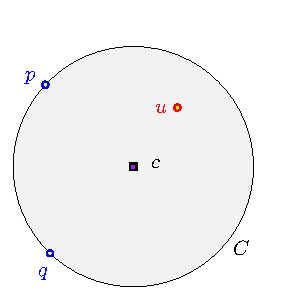
\includegraphics[page=1]{figs/shrink}%
            \hfill%
            \includegraphics[page=2]{figs/shrink}%
            \hfill%
            \includegraphics[page=3]{figs/shrink}%
            \hfill%
            \phantom{}%
            \caption{}
            \figlab{shrink}
        \end{figure}
        \item $m >0$: Let $\pc\in \PS$ be a point in the interior of
        $\disk$. We move the center $\cen$ of $\disk$ in the direction
        of $\pa$, shrinking $\disk$ in the process, so that the radius
        the disk is $\dY{\cen}{\pa}$, until we get a disk
        $\disk' \subseteq \disk$ such that $\pc$ is on the boundary of
        $\disk'$, see \figref{shrink}. Observe that $\pa$ and $\pc$
        are on the boundary of the new disk, and
        $|\interiorX{\disk'} \cap \PS| < |\interiorX{\disk} \cap
        \PS|$. Thus, by induction, there is a path $\gamma'$ between
        $\pa$ and $\pc$ in
        $\restrictY{\DT}{\disk'} \subseteq
        \restrictY{\DT}{\disk}$. Similarly, there must be a path
        $\gamma''$ between $\pc$ and $\pb$, and concatenating the two
        paths results in a path between $\pa$ and $\pb$ in
        $\restrictY{\DT}{\disk}$.
    \end{compactitem}
    \medskip%
    \noindent
    Back to the original claim.  For any two points
    $\pa,\pb \in \disk \cap \PS$ one can get a disk
    $\disk' \subseteq \disk$ that contains $\pa$ and $\pb$ on its
    boundary.  Indeed, shrink the radius of $\disk$ till, say, $\pa$
    is on the boundary, and them move the center of the disk towards
    $\pa$ while shrinking the size of the disk to maintain $\pa$ on
    the boundary, until $\pb$ is also on the boundary of the shrank
    disk.
\end{proof}



%%%%%%%%%%%%%%%%%%%%%%%%%%%%%%%%%%%%%%%%%%%%%%%%%%%%%%%%%%%%%%%%%%%%%%%%%
\subsection{The construction of local spanners for disks}

\subsubsection{The construction}

The input is a set $\PS$ of $n$ points in the plane (in general
position) with $\spread = \spreadX{\PS}$, and a parameter
$\eps \in (0,1)$.

The algorithm computes a $1/\epsA$-\WSPD $\WS$ of $\PS$ using the
algorithm of \lemref{s:s:p:d:spread}, where $\epsA = \eps/6$.  For
each pair $\Pair = \{\PSX, \PSY \} \in \WS$, the algorithm computes
the Delaunay triangulation $\DT_{\Pair} = \DTX{ \PSX \cup \PSY}$. The
algorithm adds all the edges in $\DT_{\Pair} \cap (\PSX \otimes \PSY)$
to the computed graph $\G$.

\subsubsection{Analysis}

\paragraph{Size.}

For each pair $\Pair = \{\PSX, \PSY\}$ in the \WSPD, its Delaunay
triangulation contains at most with $O( |\PSX| + |\PSY|)$ edges. As
such, the number of edges in the resulting graph is bounded by
\begin{equation*}
    \sum_{\{\PSX, \PSY\} \in \WS} O\bigl( |\PSX| + |\PSY| \bigr)
    =%
    O\pth{ \WeightX{\WS} }%
    =%
    O\pth{ \frac{n\log \spread}{{\epsA}^{2}}},
\end{equation*}
by \lemref{s:s:p:d:spread}.


\paragraph{Construction time.}
The construction time is bounded by
\begin{equation*}
    \sum_{\{\PSX, \PSY\} \in \WS} O\bigl( (|\PSX| + |\PSY|) \log
    (|\PSX| + |\PSY|)  \bigr)
    =%
    O\pth{ \WeightX{\WS} \log n }%
    =%
    O\pth{ \frac{n\log \spread \log n}{{\epsA}^{2}}},    
\end{equation*}

\paragraph{Local spanner property.}

\begin{lemma}
    Let $\G$ be the graph constructed above for the point set
    $\PS$. Then, for any (close) disk $\disk$, and any two points
    $\px, \py \in \PS \cap \disk$, we have that
    $\restrictY{\G}{\disk}$ has a $(1+\eps)$-path between $\px$ and
    $\py$. That is, $\G$ is a $(1+\eps)$-local spanner for disks.
\end{lemma}

\begin{proof}
    The proof is by induction on the distance between $\pa$ and $\pb$
    (or more precisely, the rank of their distance among the
    $\binom{n}{2}$ pairwise distances).  Consider the pair
    $\Pair = \{ \PSX, \PSY \}$ such that $\px \in \PSX$ and
    $\py \in \PSY$.

    For the base case, consider the case that $\px$ is the
    nearest-neighbor to $\py$ in $\PS$, and $\py$ is the
    nearest-neighbor to $\px$ in $\PS$.  It must be, because of the
    separation property of $\Pair$, that $\PSX$ and $\PSY$ are
    singletons. Indeed, if $\PSX$ contains another point, then $\py$
    would not be the nearest-neighbor to $\px$ (this is true for
    $\epsA < 0.5$). As such, $\px \py \in \DT_\Pair$,
    $\px, \py \in \disk$, and the edge $\px \py \in \EGX{\G}$,
    implying the claim.

    For the inductive step, observe that , the claim follows if
    $\px \py \in \DT_\Pair$, so assume this is not the case. By the
    connectivity of $\DT_\Pair \cap \disk$, see
    \clmref{d:t:connected}, there must be points
    $\px' \in \PSX \cap \disk$, $\py' \in \PSY \cap \disk$, such that
    $\px'\py' \in \EGX{ \DT_\Pair}$. As such, by construction, we have
    that $\px'\py' \in \EGX{\G}$. Furthermore, by the separation
    property, we have that    
    \begin{equation*}
        \max \pth{ \diameterX{\PSX}, \diameterX{\PSY} }%
        \leq%
        \epsA \cdot \DistSetY{\PSX}{\PSY}%
        \leq%
        \epsA \ell, 
    \end{equation*}
    where $\ell = \dY{\px}{\py}$. In particular,
    $\dY{\px'}{\px} \leq \epsA \ell$ and
    $\dY{\py'}{\py} \leq \epsA \ell$. As such, by induction, we have
    $\dGZ{\G}{\px}{\px'} \leq (1+\eps)\dY{\px}{\px'} \leq
    (1+\eps)\epsA \ell$ and
    $\dGZ{\G}{\py}{\py'} \leq (1+\eps)\dY{\py}{\py'} \leq
    (1+\eps)\epsA \ell$.  Furthermore,
    $\dY{\px'}{\py'} \leq (1+2\epsA)\ell$. As $\px'\py' \in \EGX{\G}$,
    we have
    \begin{align*}
      \dGZ{\G}{\px}{\py}%
      &\leq%
        \dGZ{\G}{\px}{\px'}%
        +\dY{\px'}{\py'}
        +
        \dGZ{\G}{\py'}{\py}%
        \leq%
        (1+\eps)\epsA \ell
        +(1+2\epsA)\ell
        + (1+\eps)\epsA \ell
        \leq%
        \pth{ 2\epsA +1+2\epsA + 2\epsA } \ell        
      \\&%
      =%
      \pth{ 1+ 6\epsA  } \ell        
      \leq%
      \pth{ 1+ \eps  } \dY{\px}{\py},
    \end{align*}
    if $\epsA \leq \eps/6$.
\end{proof}

\paragraph{The result.}

\begin{theorem}
    \thmlab{main:1}%
    %
    Let $\PS$ be a set of $n$ points in the plane, and let
    $\eps \in (0,1)$ be a parameter. The above algorithm constructs a
    local $(1+\eps)$-spanner $\G$ for disks. The spanner has
    $O\pth{ \eps^{-2} n\log \spread }$, with running time
    $O\pth{ \eps^{-2} n\log \spread \log n }$.  Formally, for any disk
    $\disk$ in the plane, and any two points
    $\pa, \pb \in \PS \cap \disk$, we have a $(1+\eps)$-path in
    $\restrictY{\G}{\disk}$.
\end{theorem}

% ------------------------------------------------------------------------
\subsubsection{Applications and comments}


\begin{defn}
    Given a region $R$ in the plane and a point set $\PS$, consider
    two points $\pa, \pb \in \PS$. The edge $\pa \pb$ is \emphw{safe}
    in $R$, if there is a disk $\disk$ such that
    $\pa,\pb \in \disk \subseteq R$. Let $\GY{\PS}{R}$ be the graph
    formed by all the safe edges in $\PS$ for $R$. Note, that his
    graph might have a quadratic number of edges in the worst case.
\end{defn}

Observe that $\GY{\Re^2}{\PS}$ is a clique.

\begin{corollary}
    Let $\PS$ be a set of $n$ points in the plane, and let
    $\eps \in (0,1)$ be a parameter, and let $\G$ be a local
    $(1+\eps)$-spanner for disks. Then, for $R$ be an region in the
    plane, and consider the graph $\GA = \GY{\PS}{R}$. Then
    $\restrictY{\G}{R}$ is a $(1+\eps)$-spanner for
    $\restrictY{\GA}{R}$. Formally, for any two points
    $\pa, \pb \in \PS \cap R$, we have that
    $\dGZ{\GA}{\pa}{\pb} \leq (1+\eps)\dGZ{\G}{\pa}{\pb}$.

    In particular, for any convex region $C$, the graph $\G \gminus C$
    is a $(1+\eps)$-spanner for $\GY{\Re^2}{\PS} \gminus C$.
\end{corollary}
\begin{proof}
    Consider the shortest path $\pi = u_1 u_2 \ldots u_k$ between
    $\pa$ and $\pb$ in $\dGZ{\GA}{\pa}{\pb}$. Every edge
    $e_i = u_i u_{i+1}$ has a disk $\disk_i$ such that
    $u_i, u_{i+1} \in \disk_i \subseteq R$. As such, there is a
    $(1+\eps)$-path between $u_i$ and $u_{i+1}$ in
    $\restrictY{\G}{\disk_i} \subseteq
    \restrictY{\G}{R}$. Concatenating these paths directly yields the
    desired result.

    The second claim follows by observing that the complement of $C$
    is the union of halfspaces, and halfspaces can be considered to be
    ``infinite'' radius disks. As such, the above argument applies
    verbatim.
\end{proof}

\paragraph{But why not \SSPD?}

The result of \thmref{main:1} is somewhat disappointing as it depends
on the spread of the point set (logarithmically, but still). A natural
way is to try and emulate the construction of Abam \etal
\cite{abfg-rftgs-09} and use \SSPD instead of \WSPD. The total weight
of the \SSPD is near linear (with no dependency on the
spread). Furthermore, after some post processing, one can assume every
pair $\Pair = \{ \PSX, \PSY \}$ is angularly $\eps$-separated -- that is,
there is a double wedge with angle $\leq \eps$, such that $\PSX$ and
$\PSY$ are of different sides of the double wedge. The problem is that
for the local disk $\disk$, it might be
the bridge edge between $\PSX$ and $\PSY$ that is in $\DT_\Pair \cap
\disk$ is much longer than the two points of interest. This somewhat
counter-intuitive situation is illustrated in \figref{bad}.

\begin{figure}[h]
    \phantom{}
    \hfill%
    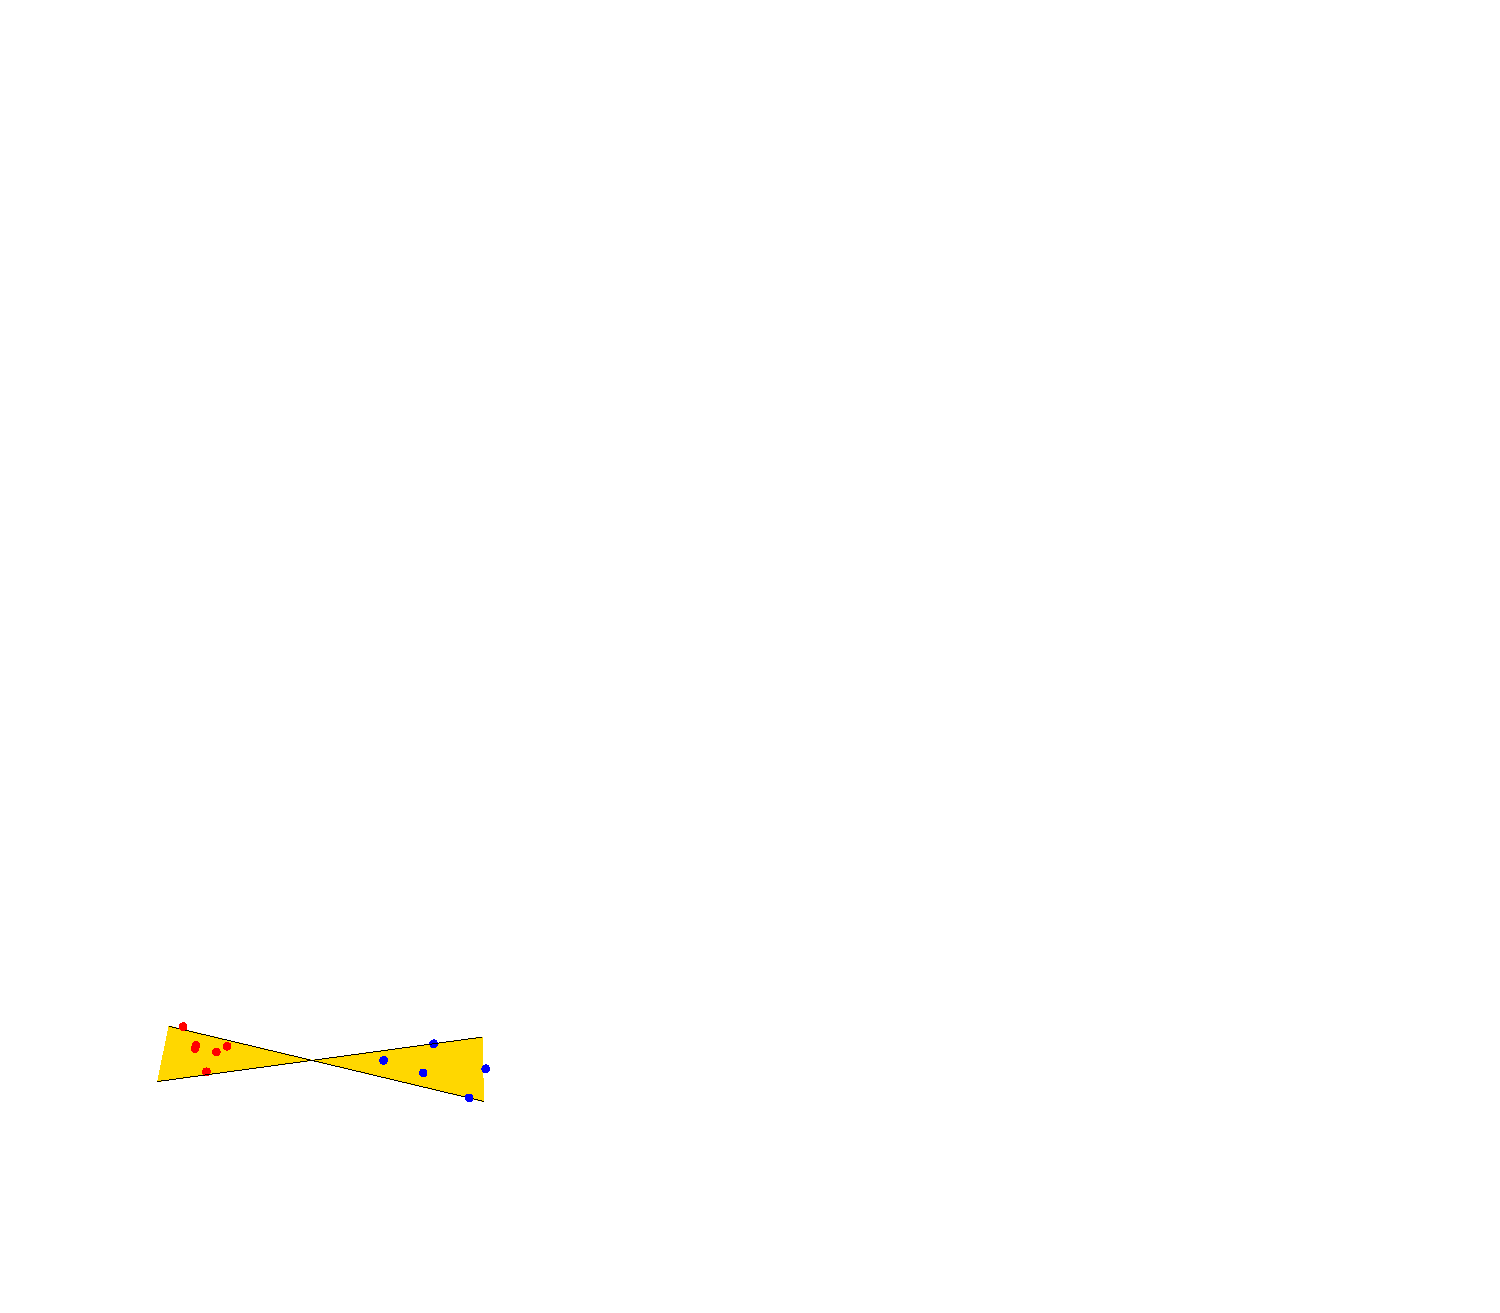
\includegraphics[page=1]{figs/bad_example}
    \hfill%
    \includegraphics[page=2]{figs/bad_example}
    \hfill%
    \includegraphics[page=3]{figs/bad_example}
    \hfill%
    \phantom{}
    \caption{A bridge too far -- the only surviving bridge between the
       red and blue points is too far to be useful if the sets are
       points are not well separated.}
    \figlab{bad}
\end{figure}



%%%%%%%%%%%%%%%%%%%%%%%%%%%%%%%%%%%%%%%%%%%%%%%%%%%%%%%%%%%%%%%%%%%%%%%%%
%%%%%%%%%%%%%%%%%%%%%%%%%%%%%%%%%%%%%%%%%%%%%%%%%%%%%%%%%%%%%%%%%%%%%%%%%
%%%%%%%%%%%%%%%%%%%%%%%%%%%%%%%%%%%%%%%%%%%%%%%%%%%%%%%%%%%%%%%%%%%%%%%%%


\subsection{A local spanner for axis parallel squares}

One can modify the above construction for axis-parallel squares, and
get a local spanner without dependency on the spread.  In the
following we assume that the point set $\PS$ is in general position --
no two points share a coordinate value, or appear in opposing corners
of an axis-parallel square -- this can be ensured by slightly
perturbing the points if necessary.

We need the following simple lemma.

\begin{lemma}
    (A) Let $\sqr$ be an axis parallel square in the plane, and let
    $\pa, \pb$ be two arbitrary points in $\sqr$. Then, there is a
    square $\sqrA \subseteq \sqr$ that contains $\pa$ and $\pb$ on its
    boundary.

    (B) Let $\PSX, \PSY$ be two point sets in the plane, such that
    $\PSX' = \PSX \cap \sqr \neq \emptyset$ and
    $\PSY' = \PSY \cap \sqr \neq \emptyset$. Let
    $\px \in \PSX, \py \in \PSY$ be the two points realizing
    $\dsZ{\infty}{\PSX'}{\PSY'} = \min_{\pa \in \PSX', \pb \in \PSY'}
    \dZ{\infty}{\pa}{\pb}$. Then, there is a square
    $\sqrA \subseteq \sqr$ that contains $\px$ and $\py$ on its
    boundary, and $\sqrA$ does not contain any other point of
    $\PSX \cup \PSY$.
\end{lemma}
\begin{proof}
    (A) Start shrinking $\sqr$ around its center till it contains one
    of the points (say $\pa$ on its boundary. Next, move the center of
    the square towards $\pa$ till the boundary of the continuously
    shrinking square passes through $\py$. If $\px$ and $\py$ lies on
    adjacent face, then continue the shrinking process by moving the
    center towards the common corner of the shared edges -- this
    process stops when one of the points is on the corner of the
    square.  Clearly, the resulting square $\sqrA$ is the desired
    square.


    (B) Let $r = \dsZ{\infty}{\PSX'}{\PSY'}$. By (A), there is a
    square $\sqrA \subseteq \sqr$ having $\px$ and $\py$ on apposing
    sides. As such, the sidelength of $\sqrA$ is $r$. Assume for
    contradiction, that there is some other point
    $\px' \in \PSX \cap \sqrA$. By our general position assumption,
    $\px'$ is in the interior of $\sqrA$, and in particular,
    $\dZ{\infty}{\px'}{\py} < r$, which is a contradiction to the
    choice of $\px$ and $\py$.
\end{proof}
XXX



\begin{lemma}
    \lemlab{squares}%
    %
    Let $\PS$ be a set of $n$ points in the plane, and let
    $\eps \in (0,1)$ be a parameter. A variant of the above algorithm
    constructs a local $(1+\eps)$-spanner $\G$ for axis-parallel
    squares. The spanner has $O\pth{ \eps^{-3} n \log n }$ edges, and
    the construction time is
    $O\pth{ \eps^{-3} n\log \spread \log n }$.  Formally, for any axis
    parallel square $\sqr$ in the plane, and any two points
    $\pa, \pb \in \PS \cap \sqr$, we have a $(1+\eps)$-path in
    $\restrictY{\G}{\sqr}$.
\end{lemma}
\begin{proof}
    One can define the Delaunay triangulation when the unit ball is
    replaced by the unit square. Formally, in this triangulation two
    points are connected $\iff$ there is a square that contains these
    two points on its boundary and no points in its interior. Let
    $\DT_\square$ denote the resulting Delaunay triangulation. Instead
    of constructing a \WSPD, the algorithm computes a $1/\epsA$-\SSPD
    $\WS$. Increasing the weight and number of pairs by a factor of
    $O(1/\epsA)$, one can assume that every pair
    $\{ \PSX, \PSY \} \in \WS$ is not only semi-separated, but also
    there is an associated double wedge of angle $\leq \epsA$, the
    left pane in \figref{bad}. The algorithm now computes the
    ``square'' Delaunay triangulation for each such pair, and add the
    edges of the triangulation to the resulting graph $\G$.

    The proof that the spanner property holds in this case is somewhat
    more involved, which we will mitigate by being more sketchy about
    the details. As before, consider two points
    $\px, \py \in \PS \cap \sqr$, where $\sqr$ is some arbitrary
    square. Let $\sqrA$ be the smallest square containing these two
    points. The points $\px$ and $\py$ are on opposing edges of
    $\sqr'$ (potentially one of them is in a corner). Let
    $\PSX' = \PSX \cap \sqr'$ and $\PSY' = \PSY \cap \sqr'$, and
    consider the two points $\px' \in \PSX'$ and $\py' \in \PSY'$
    realizing $\DistSetY{\PSX'}{\PSY'}$ (under the $L_\infty$
    norm). The key observation is that there is a square $\sqrA$
    containing the two points on its boundary, such that
    $\sqrB \subseteq \sqrA$ and $\sqrA$ contains no other points
    $\PSX \cup \PSY$ (this shrinking property does not hold in the
    disk case). That is -- $\px' \py' \in \G$. Assume, that
    $\diameterX{\PSX} < \diameterX{\PSY}$, which implies that
    $\dY{\px}{\px'} \leq \diameterX{\PSX} \leq \epsA
    \DistSetY{\PSX}{\PSY} \leq \epsA \dY{\px'}{\py'}$. A tedious but
    straightforward calculation shows that
    $\dY{\py'}{\py} < \dY{\px}{\py}$, One can now use induction to
    argue that $\dGZ{\G}{\py'}{\py} \leq (1+\epsA)
    \dY{\py'}{\py}$. One can now use that the two point sets are
    inside the narrow double wedge to argue that
    $\dGZ{\G}{\px}{\py} \leq \bigl(1+O(\epsA)\bigr)\dY{\px}{\py}$,
    which implies the claim.

    \sariel{Too sketchy -- to add details... And a figure.}

    ~
\end{proof}

\subsection{Result for other norms}

\subsubsection{The rest}

\sariel{FILL IN *all* THE DETAILS -- this is way too hand wavy --
   including refs, etc}

Using the same argument, we can extend the result for the case where
$\LL$ is the set of all scaled and translated copies, homothets, of a
convex shape $\CC$. While the Delaunay triangulation is not well
defined for all convex shapes, the operation of creating edges between
two points $p,q\in P$ such that there exist a homothet of $\CC$ that
contains only $p$ and $q$ and no other point of $\PS$ is always well
defined, and gives us a graph known as the $\CC$-Delaunay graph of
$\PS$, and denoted $\DG_{\CC}(P)$. The above proof applies almost
verbatim for any convex $\CC$, and proves the connectivity of
$\DG_{\CC}(P)$ for any $L\in \LL$.

We need only to define a suitable shrinking operation for convex
region towards a point, which is possible, for example, by
parameterizing the curve defining the region and leaving the desired
point in the same coordinate of the smaller curve. So, we get a
$(1+\eps)-\LL$ local spanner of size $O(\eps^{-3}n\log n)$ in
$O(\eps^{-2}n\log n)$ time.(


%%%%%%%%%%%%%%%%%%%%%%%%%%%%%%%%%%%%%%%%%%%%%%%%%%%%%%%%%%%%%%%%%%%%%%%%%
%%%%%%%%%%%%%%%%%%%%%%%%%%%%%%%%%%%%%%%%%%%%%%%%%%%%%%%%%%%%%%%%%%%%%%%%%
%%%%%%%%%%%%%%%%%%%%%%%%%%%%%%%%%%%%%%%%%%%%%%%%%%%%%%%%%%%%%%%%%%%%%%%%%

\section{Axis parallel rectangles}

We would like to build local spanners (of subquadratic size) for
axis-parallel rectangles, but as \figref{bad:rectangles} shows, there
is no hope of achieving this. As such, we need to change the
requirement somewhat.

\begin{figure}
    \centerline{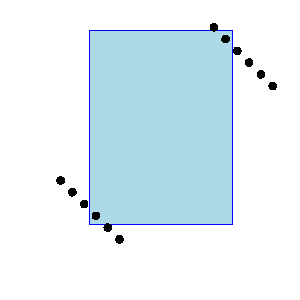
\includegraphics{figs/local_rectangles}}
    \caption{There are quadratic number of pairs of points that has to
       be connected in any local spanner for axis parallel
       rectangles. Indeed, for any point in the top diagonal and
       bottom diagonal, there is an axis parallel rectangle that
       contains only these two points. This holds even if we restrict
       ourselves to fat rectangles of similar size.}
    \figlab{bad:rectangles}
\end{figure}


\paragraph{A weaker connectivity requirement.}

For a rectangle $\rect$, let $(1-\delta)\rect$ denote the rectangle
resulting from scaling $\rect$ by a factor of $1-\delta$ around its
center. For a point set $\PS$ in the plane, a graph $\G =(\PS,\EG)$ is
a \emphi{$(1-\delta)$-local $(1+\eps)$-spanner} for $\PS$, if for any
axis parallel rectangle $\rect$, we have that $\restrictY{\G}{\rect}$
is an $\eps$-spanner for any two points in $(1-\delta)\rect \cap
\PS$. Intuitively, the spanner does not need to work for points that
are close to the boundary of $\rect$. We refer to
$\rect \setminus (1-\delta)\rect$ as the \emphi{shadow} of $\rect$ --
it is the area that is being damaged, and that the local spanner fails
to work for.

Before dwelling into the construction, we start with presenting a new
pair decomposition that would be useful for our (nefarious) purposes.



\subsection{Quadrant separated pairs decomposition}

For points $\pa = (p_1, \ldots, p_d)$ and $\pb = (q_1, \ldots, q_d)$
in $\Re^d$, let $\pa \prec \pb$ denotes that $\pb$ \emphi{dominates}
$\pa$ coordinate-wise. That is $p_i < q_i$, for all $i$. More
generally, let $\pa <_i \pb$ denote that $\pa_i < \pb_i$. For two
point sets $\PSX, \PSY \subseteq \Re^d$, we use $\PSX <_i \PSY$ to
denote that $\forall \px \in \PSX, \py \in \PSY \quad \px <_i \py$.
In particular $\PSX$ and $\PSY$ are \emphw{$i$-coordinate separated}
if $\PSX <_i \PSY$ or $\PSY <_i \PSX$. A pair $\{ \PSX, \PSY\}$ is
\emphi{quadrant-separated}, if $\PSX$ and $\PSY$ are $i$-coordinate
separated, for $i=1,\ldots, d$.

A \emphi{quadrant-separated pairs decomposition} of a point set
$\PS \subseteq \Re^d$, is a pairs decomposition (see
\defref{pair:decomposition}
$\WS = \bigl\{ \{ \PSX_1, \PSY_1 \}, \ldots, \{ \PSX_s, \PSY_s \}
\bigr\}$ of $\PS$, such that $\{ \PSX_i, \PSY_i\}$ are
quadrant-separated for all $i$.


\begin{lemma}
    \lemlab{d:1}%
    %
    Given a set $\PS$ of $n$ points in $\Re$, one can compute, in
    $O( n \log n)$ time, a \QSPD of $\PS$ with $O(n)$ pairs, and of
    total weight $O( n \log n)$.
\end{lemma}
\begin{proof}
    If $\PS$ is a singleton then there is nothing to do. If
    $\PS = \{ \pa, \pb \}$, then the decomposition is the pair formed
    by the two singleton points.

    Otherwise, let $x$ be the median of $\PS$, such that
    $\PS_{\leq x} = \Set{ \pa \in \PS }{\pa \leq x}$ contains exactly
    $\ceil{n/2}$ points, and $\PS_{> x} = \PS \setminus \PS_{\leq x}$
    contains $\floor{n/2}$ points. Construct the pair
    $\Pair = \{ \PS_{\leq x}, \PS_{> x} \}$, and compute recursively a
    \QSPD{}s $\QS_{\leq x}$ and $\QS_{> x}$ for $\PS_{\leq x}$ and
    $\PS_{> x}$, respectively. The desired \QSPD is
    \begin{math}
        \QS_{\leq x} \cup \QS_{> x} \cup \{ \Pair \}.
    \end{math}
    The bounds on the size and weight of the desired \QSPD are
    immediate.
\end{proof}


\begin{lemma}
    Given a set $\PS$ of $n$ points in $\Re^d$, one can compute, in
    $O( n \log^d n)$ time, a \QSPD of $\PS$ with $O(n \log^{d-1} n)$
    pairs, and of total weight $O( n \log^d n)$.
\end{lemma}
\begin{proof}
    The construction algorithm is recursive on the dimensions, using
    the algorithm of \lemref{d:1} in one dimension.

    The algorithm computes a value $\alpha_d$ that partition the
    values of the points in $d$\th coordinate roughly equally (and is
    distinct from all of them), and let $h$ be a hyperplane parallel
    to the first $d-1$ coordinate axes, and having value $\alpha_d$ in
    the $d$\th coordinate.

    Let $\PS_{\uparrow}$ and $\PS_{\downarrow}$ be the subset of
    points of $\PS$ that are above and below $h$, respectively.  The
    algorithm computes recursively \QSPD{}s $\QS_\uparrow$ and
    $\QSdown$ for $\PSup$ and $\PS_{\downarrow}$, respectively.  Next,
    the algorithm projects the points of $\PS$ to $h$, and let $\PS'$
    be the resulting $d-1$ dimensional point set (after we ignore the
    $d$\th coordinate). Compute recursively a \QSPD $\QS'$ for $\PS'$.

    
    For a point set $\PSX' \subseteq \PS'$, let $\liftX{\PSX'}$ be the
    subset of points of $\PS$ that its projection to $h$ is $\PSX'$.
    The algorithm now computes the set of pairs
    \begin{equation*}
        \widehat{\QS}%
        =%
        \Set{\Bigl.
           \{ \liftX{ \PSX'} \cap \PSup , \liftX{ \PSY' } \cap \PSdown
           \}, \,\,
           \{ \liftX{ \PSX'} \cap \PSdown , \liftX{ \PSY' } \cap \PSup
           \}
        }%
        { \{ \PSX', \PSY' \} \in \QS'}     .
    \end{equation*}
    The desired \QSPD is $\widehat{\QS} \cup \QSup \cup \QSdown$.

    To observe that this is indeed a \QSPD, observe that all the pairs
    in $\QSup, \QSdown$ are quadrant separated by induction. As for
    pairs in $\widehat{\QS}$, they are quadrant separated in the first
    $d-1$ coordinates by induction on the dimension, and separated in
    the $d$ coordinate since one side of the pair comes from $\PSup$,
    and the other side from $\PSdown$.

    As for coverage, consider any pair of points $\pa, \pb \in \PS$,
    and observe that the claim holds by induction if they are both in
    $\PSup$ or $\PSdown$. As such, assume that $\pa \in \PSup$ and
    $\pb \ni \PSdown$. But then there is a pair
    $\{\PSX', \PSY'\} \in \QS'$ that separates the two projected
    points in $h$, and clearly one of the two lifted pairs that
    corresponds to this pair quadrant-separates $\pa$ and $\pb$ as
    desired.

    The number pairs in the decomposition is
    \begin{math}
        N(n,d) = 2N(n,d-1) + 2N\pth{ n/2, d }
    \end{math}
    with $N(n,1) = O(n)$. The solution to this recurrence is
    $N(n,d) = O( n \log^{d-1} n)$.
    The total weight of the decomposition is
    \begin{math}
        W(n,d) = 2W(n,d-1) + 2W\pth{ n/2, d }
    \end{math}
    with $W(n,1) = O(n \log n)$. The solution to this recurrence is
    $W(n,d) = O( n \log^{d} n)$. Clearly, this also bounds the
    construction time.
\end{proof}


\subsection{Bounded aspect ratio rectangles}
Let $\LL$ be the set of axis parallel rectangles with aspect ratio at
most $1<\alpha$. We repeatedly preform the algorithm for convex local
spanners with rectangles of different aspect-ratio, where in the
$i$\th iteration we use a rectangle with aspect ratio
$\left(1+\eps\right)^i$, where $i\in\{0,...,\log_{1+\eps}(\alpha)\}$.

Let $r$ be a rectangle with aspect ratio $\alpha$, and let $(A,B)$ be
a pair in an SSPD such that $A\cap r\neq \emptyset$, and
$B\cap r\neq \emptyset$. We assume w.l.o.g that the height of $r$ is
1, and its width is $\alpha'\in [1,\alpha]$.

Let $i\in \{0,...,\log_{1+\eps}(\alpha)\}$ be an index for which
$\alpha' \leq (1+\eps)^i \leq \frac{\alpha}{1-\eps}$ if such an index
exists, then let $r'$ be the rectangle with width $\alpha'$ and aspect
ratio $(1+\eps)^i$, whose horizontal bisector coincides with that of
$r$. Since $(1+\eps)^i \leq \frac{\alpha}{1-\eps}$, we have that
$r\setminus r'$ is contained within the shadow of $r$, and therefore
$r'$ contains points of both $A$ and $B$, from the correctness of the
convex local spanner, we will have an edge between a point in
$A\cap r'$ and a point in $B\cap r'$. As before, this, together with
the properties of the SSPD, is enough to guarantee that the
constructed graph is indeed a $(\LL, \eps)$-$t$-spanner (for the
appropriate choice of the parameter $s$ of the SSPD).

We are left with proving that there exists an index
$i\in \{0,...,\log_{1+\eps}(\alpha)\}$ for which
$\alpha' \leq (1+\eps)^i \leq \frac{\alpha}{1-\eps}$.




\begin{equation}
    \alpha' \leq (1+\eps)^i \leq \frac{\alpha}{1-\eps}
\end{equation}

\begin{equation}
    \log_{1+\eps}(\alpha') \leq i \leq
    \log_{1+\eps}\left(\frac{\alpha}{1-\eps}\right)
\end{equation}

\begin{equation}
    \log_{1+\eps}(\alpha') \leq i \leq \log_{1+\eps}(\alpha) -
    \log_{1+\eps}(1-\eps)
\end{equation}

\hrule

If $\log_{1+\eps}(1-\eps)<-1$, then there must be an integer $i$ with
the required properties. We now notice that
$(1+\eps)^{-1}=\frac{1}{1+\eps}>(1-\eps)$ [since
$1>(1-\eps)(1+\eps)=(1-\eps^2)$], and so $i$ exists.

The size of the spanner is $\log_{1+\eps}(\alpha)$ times the number of
edges in a convex local spanner, and since
$\log_{1+\eps}(\alpha)=O\left(\frac{\log(\alpha)}{\eps}\right)$, we
have a spanner of size
$O\left(\frac{\log(\alpha)}{\eps (t-1)^{-3}}n\log n\right)$


\subsection{Arbitrary rectangles}

In order to construct local spanners for the family $\LL$ of axis
parallel rectangles with $\eps$-shadow, we describe a decomposition of
the point set $P\subseteq \Re^2$ in to pairs of sets, a decomposition
which we name a Quadrant Separated Pair Decomposition (\QSPD). This
decomposition gives us $O(n\log^2n)$ pairs $(A_i,B_i)$ of subsets of
$\PS$, such that the sets can be separated by a vertical line and also
by a horizontal line, and for every two points $p,q\in P$, there
exists a single pair $(A_i,B_i)$ such that (w.l.o.g) $p\in A_i$,
$q\in B_i$. This separation can be viewed as if on of the sets lies in
the first quadrant of the plane (i.e. every point has positive $x$ and
$y$ values), and the other is in the third quadrant (i.e. every point
has negative $x$ and $y$ values), hence the name.

The construction of the decomposition can be described as the repeated
recursive invocation of two fairly simple subroutines denoted $S_1$
and $S_2$. The first subroutine $S_1$ goes as follows. Given a set of
points $\PS$, and a horizontal line $l_y$, find the median of $\PS$
w.r.t. the $x$-coordinates of the points, and create the vertical line
$l_x$ passing through it. $l_x$ and $l_y$ now divide the plane into 4
quadrants, add both pairs of diagonally opposing quadrants to the
decomposition, and recurse twice, once on the points to the left of
$l_x$, and once on the points to its right.

The second operation is now even easier to describe. Find the median
of $\PS$ w.r.t. the $y$-coordinates of the points, create the
horizontal line $l_y$ passing through that point, call $S_1(P,l_y)$,
and recurse twice, once on the points to below of $l_y$, and once on
the points above it.

\begin{claim}
    The subroutine $S_2(P)$ creates a \QSPD with size $O(n\log^2n)$.
\end{claim}

\begin{proof}
    By construction, each reported pair is separated w.r.t. to both
    dimensions, and any two point appear in diagonally opposing
    quadrants exactly once, as every recursive calls to both $S_1$ and
    $S_2$ will include only one of the points.
    
    Every call to $S_1$ creates two pairs, and generates two recursive
    calls, each with exactly half of the points. The formula for the
    size of the pairs created by $S_1$ is therefore
    $T(n)=2T\left( \frac{n}{2}\right) + O(n)$, which solves to
    $O(n)$. Very similarly, each call to $S_2$ calls $S_1$ once, and
    generates two recursive calls, each with exactly half of the
    points. The total number of pairs is therefore
    $S(n)=2S\left( \frac{n}{2}\right) + O(n\log n)$, which solves to
    $O(n\log^2n)$.
    
\end{proof}






We first describe a subroutine for connecting two sets of points, $A$
and $B$, where $A$ is contained in $Q^-$, the negative quadrant of the
plane (i.e., have a negative value $x$-coordinate and a negative value
$y$-coordinate), and $B$ is contained in $Q^+$, the positive quadrant
of the plane.

Our algorithm will connect every point in $A$ to
$O\left(\frac{1}{\eps^2}\right)$ points in the positive quadrant, and
after performing the same process for the points of the symmetrically
defined $B'$, we will have that every rectangle that truly contains
points from $A$ and $B$ will have an edge $(a,b)$ with $a\in A$ and
$b\in B$.

For every point $a = (x',y') \in A$ we define partition the positive
quadrant into $O\left(\frac{1}{\eps^2}\right)$ sets. We consider the
following $\frac{1}{\eps}$ horizontal stripes -
$\forall j\in \{1,...,\frac{1}{\eps}\}$:

\hrule

If $\log_{1+\eps}(1-\eps)<-1$, then there must be an integer $i$ with
the required properties. We now notice that
$(1+\eps)^{-1}=\frac{1}{1+\eps}>(1-\eps)$ [since
$1>(1-\eps)(1+\eps)=(1-\eps^2)$], and so $i$ exists.

The size of the spanner is $\log_{1+\eps}(\alpha)$ times the number of
edges in a convex local spanner, and since
$\log_{1+\eps}(\alpha)=O\left(\frac{\log(\alpha)}{\eps}\right)$, we
have a spanner of size
$O\left(\frac{\log(\alpha)}{\eps (t-1)^{-3}}n\log n\right)$

\subsection{Q{}S{}PD}
Implementing a motion planning algorithm that created a road-map of
both free space and obstacle space by simulating probe queries to near
obstacles and using those to execute a space exploration algorithm.
After a basic algorithm is implemented and tested, our goals will
include extending the algorithm for the case of dynamic obstacles, and
optimization of the data structure at the base of the algorithm.

In order to construct local spanners for the family $\LL$ of axis
parallel rectangles with $\eps$-shadow, we describe a decomposition of
the point set $P\subseteq \Re^d$ in to pairs of sets, a decomposition
which we name a Quadrant Separated Pair Decomposition (\QSPD). This
decomposition gives us $O(n\log^{d-1}n)$ pairs $(A_i,B_i)$ of subsets
of $P$, with overall size $O(n\log^{d}n)$, such that the sets can be
separated by $d$ orthogonal axis parallel hyperplanes, and for every
two points $p,q\in P$, there exists a single pair $(A_i,B_i)$ such
that (w.l.o.g) $p\in A_i$, $q\in B_i$. For clarification, this
separation in $\Re^d$ can be viewed as if one of the sets lies in the
first quadrant of the plane (i.e. every point has positive $x$ and $y$
values), and the other is in the third quadrant (i.e. every point has
negative $x$ and $y$ values), hence the name.

The construction of the decomposition can be described as a recursive
process in which a call to the function with $p\subseteq \Re^d$ of
size $n$ invokes a single call to a lower dimensional case, and two
calls to $d$-dimensional cases, each with half of the points. The
function goes as follows.

Given a set $P\subseteq \Re^d$ and a coloring
$c:P\longrightarrow \{0,1\}^k$ for some $k$, the function $f(P,c)$
finds a median of $P$ w.r.t. the $d$\th dimension, and projects the
points $P$ onto a hyperplane $h$ orthogonal to the same dimension
passing through the median. Let the projected set of points be denoted
$P'$, the $\frac{n}{2}$ points of $P$ the lie above $h$ be denoted
$P^+$, $P\setminus P^+$ be denoted $P^-$, and let $c'$ be the coloring
defined by $c'(p)=c(p)\oplus b$ where $\oplus$ is the concatenation
operator, and $b=1$ if $p\in P^+$, and $p=0$ otherwise.

The function then calls $f(P', c')$, $f(P^+, c^+)$, and $f(P^-, c^-)$,
where $c^+$ and $c^-$ are $c$ limited to the set $P^+$ and $P^-$
respectively.

In the case where $d=1$, after finding the median w.r.t. the single
dimension and defining $c'$, instead of invoking a lower dimensional
call, the function creates $2^{d-1}$ pairs by taking all of the points
with the same value $x\in\{0,1\}^d$ under $c'$, and pairing that set
with the set all of the points with value $y\in\{0,1\}^d$ such that
$\forall 1\leq i\leq d~:~ x^{(i)}\neq y^{(i)}$.


\begin{claim}
    The process described above creates a \QSPD with size
    $O(n\log^dn)$ in $O_d(n\log^dn)$ time.
\end{claim}

\begin{proof}
    By construction, each reported pair is separated by $d$ orthogonal
    axis parallel hyperplanes, and any two points appear in opposing
    quadrants exactly once, as every recursive call which assigns
    different bits of the coloring to two points, separates these
    points in the next recursive calls.
	
    The size of the structure is given by the following recursion
    formula:
    \begin{equation}
        S(n,d) = S(n,d-1) + 2S\left(\frac{n}{2},d\right)
    \end{equation}
	
    In the base case where $d=1$, the formula is slightly different,
    as instead of recursing in a lower dimension it directly adds
    pairs. The formula is:
	
	\begin{equation}
            S(n,1) = O(n) + 2S\left(\frac{n}{2},1\right)
        \end{equation}
	
	which solves to $O_d(n\log n)$. This means that the general
        case is
	
	\begin{equation}
            S(n,d) = O(n\log^{d-1}n) + 2S\left(\frac{n}{2},d\right)
        \end{equation}
	
	which solves to $O(n\log^d n)$.
	
	By using $d$ sorted arrays, one for each dimension, we get
        that the same recursion formulas hold for the runtime of the
        algorithm.
    \end{proof}

    \subsection{Arbitrary rectangles}

    Let $P\subseteq \Re^2$. We first describe a subroutine for
    connecting two sets of points, $A$ and $B$, where $A$ is contained
    in $Q^-$, the negative quadrant of the plane (i.e., have a
    negative value $x$-coordinate and a negative value
    $y$-coordinate), and $B$ is contained in $Q^+$, the positive
    quadrant of the plane.

    Our algorithm will connect every point in $A$ to
    $O\left(\frac{1}{\eps^2}\right)$ points in the positive quadrant,
    and after performing the same process for the points of the
    symmetrically defined $B'$, we will have that every rectangle that
    truly contains points from $A$ and $B$ will have an edge $(a,b)$
    with $a\in A$ and $b\in B$.

    For every point $a = (x',y') \in A$ we define partition the
    positive quadrant into $O\left(\frac{1}{\eps^2}\right)$ sets. We
    consider the following $\frac{1}{\eps}$ horizontal stripes -
    $\forall j\in \{1,...,\frac{1}{\eps}\}$:

    \hrule

\begin{equation}
    H_{j}:=\{(x,y)~|~  0 \leq x \leq x'+y'  ,~ (j-1)\cdot \eps y' < y
    \leq j\cdot \eps y'\}
\end{equation}

On top of these we add similarly built vertical stripes:

\begin{equation}
    V_{i}:=\{(x,y)~|~ (j-1)\cdot \eps x' < x \leq j\cdot \eps x',~ 0
    \leq y \leq x'+y' \}
\end{equation}

\hrule

These stripes create a grid which partitions the rectangle $r$ whose
opposite corners are $(0,0)$ and $(|x'|,|y'|)$ into $\frac{1}{\eps^2}$
cells of width $\eps x$ and height $\eps y$. Formally:

\begin{equation}
    C_{i,j}:=\{(x',y')~|~  (i-1)\cdot \eps x < x' \leq i\cdot \eps x,~
    (j-1)\cdot \eps y< y' \leq j\cdot \eps y\}
\end{equation}

We now divide the parts of the stripes that lie outside of the
rectangle $r$. The horizontal stripes are divided into cells of width
$\eps(x+y)$ and height $\eps y$, and the vertical stripes are divided
into cells of width $\eps y$and height $\eps(x+y)$. The extremal cell
in each stripe may be smaller if $x$ or $y$ are not divisible by
$\eps(x+y)$. Formally:

\hrule

These stripes create a grid which partitions the rectangle $r$ whose
opposite corners are $(0,0)$ and $(|x'|,|y'|)$ into $\frac{1}{\eps^2}$
cells of width $\eps x$ and height $\eps y$. Formally:

\begin{equation}
    C_{i,j}:=\{(x',y')~|~  (i-1)\cdot \eps x < x' \leq i\cdot \eps x,~
    (j-1)\cdot \eps y< y' \leq j\cdot \eps y\}
\end{equation}

We now divide the parts of the stripes that lie outside of the
rectangle $r$. The horizontal stripes are divided into cells of width
$\eps(x+y)$ and height $\eps y$, and the vertical stripes are divided
into cells of width $\eps y$and height $\eps(x+y)$. The extremal cell
in each stripe may be smaller if $x$ or $y$ are not divisible by
$\eps(x+y)$. Formally:

\hrule

\begin{equation}
    C_{H_{i,j}}:=\{(x',y')~|~  x' + (i-1)\cdot \eps (x+y) < x' \leq x'
    + i\cdot \eps (x+y),~ (j-1)\cdot \eps y< y' \leq j\cdot \eps y\}
\end{equation}

\begin{equation}
    C_{V_{i,j}}:=\{(x',y')~|~  (i-1)\cdot \eps x < x' \leq i\cdot \eps
    x,~ y + (j-1)\cdot \eps (x+y)< y' \leq y + j\cdot \eps (x+y)\}
\end{equation}

\hrule

The entire construction can be seen in \figref{grid_construction}.

\begin{figure}
    \centering%
    \includegraphics[width=\linewidth,page=3]%
    {figs/grid_construction}%
    \figlab{grid_construction}%
    \caption{The construction of the grid for the arbitrary axis
       parallel rectangle local spanner.}
\end{figure}

\begin{claim}
    For every rectangle $r\in \LL$ and a pair $(A,B)$ of the SSPD
    s.t. $r_{1-\eps}\cap A \neq \emptyset$ and
    $r_{1-\eps}\cap B \neq \emptyset$, there are two points
    $a\in A, b\in B$ connected by an edge.
\end{claim}

\begin{proof}
    Let $A'=A\cap r_{1-\eps}, B'=B \cap r_{1-\eps}$, and let
    $p= \underset{p'}{argmax}\{||p'||_{\infty}~:~ p'\in A\cup B\}$,
    and assume w.l.o.g that $p\in A'$ and prove that there exist a
    point $q\in B'$ connected to $p$ by an edge.
    
    We take a point $q'\in B'$. Due to the choice of $p$ we have that
    one of the coordinates of $q'$ has a smaller absolute value than
    the same respective coordinate of $p$, and assume w.l.o.g that it
    is the $x$-coordinate. Now, since $\bigcup C_{i,j} \bigcup V_i$
    cover the entire part of $Q^+$ with an absolute $x$ value lower
    that that of $p$, we have that either there is an edge $\{p,q\}$
    in the graph, or there is another point $q$ in the same cell as
    $q'$. Regardless, since the cells are of width $\eps\cdot p.x$ and
    height $\eps\cdot p.y$ ,and $r$ is of width at least $p.x$ and
    height at least $p.y$, we get that the entire cell is inside $r$,
    and therefore there exists an edge as described in the claim.
    
    \hrule

    The entire construction can be seen in
    Figure~\ref{fig:grid_construction}. We can now describe the
    construction of our spanner. For $P\subseteq \Re^2$ we create a
    \QSPD of $P$, and for every pair $(A,B)$ we add an edge between
    every point $a\in A$ (and later reverse the rolls inside the pair)
    to an arbitrary point of $P$ in every cell $C_{i,j}$, to the
    leftmost point of $P$ in every $C_{H_{i,j}}$, and to the
    bottom-most point of $P$ in every $C_{V_{i,j}}$.
\end{proof}

We now prove a lemma that summarizes the properties of the resulted
graph, and which we will then use to prove that our construction
produces an $(\LL, eps)$- local $t$-spanner for the family of
arbitrary axis parallel rectangles.


\begin{claim}
    \label{clm:span_properties}
    For any two points $a,b\in P$ that are properly contained in an
    axis parallel rectangle $r$ ,and are not connected by an edge,
    there exists a point $b'\in r$ such that if w.l.o.g
    $||b-b'|| \leq ||a-c||$ then:
    \begin{enumerate}
        \item $||b-b'|| \leq 3\eps ||a-b||)$, and
        \item there is an edge between $a$ and $b'$.
    \end{enumerate}
    Additionally, the two closest points $p,q\in P$ are connected by
    an edge.
	
\end{claim}

\begin{proof}
    Let $(A,B)$ be the unique pair of the \QSPD such that w.l.o.g
    $a\in A$ and $b\in B$, $A\subseteq Q^-$, $B\subseteq Q^+$, and
    $||b||_{1} \leq ||a||_{1}$. We denote the absolute value of the
    coordinates of a point $p$ by $p.x$ and $p.y$ for the $x$ and $y$
    coordinates respectively. If $b.x \leq a.x$ and $b.y \leq a.y$,
    then by the construction, $a$ is connected to a point $b'$ in the
    cell $C_{i,j}$ containing $b$. Since the cell's dimensions are
    $\eps\cdot a.x \times \eps a.y$, we have that
    $C_{i,j}\subseteq r$, and also:
	
	\begin{equation}
            ||b-b'||\leq \sqrt{(\eps\cdot a.x)^2+(\eps\cdot
               a.y)^2}=\eps\sqrt{a.x^2+a.y^2}\leq \eps(a.x+a.y) \leq
            2\eps||a-b||
        \end{equation}
	
	regardless of the choice of $b'$, as
        $||a-b||\geq||a-(0,0)||\geq \frac{a.x+a.y}{2}$.
	
	If w.l.o.g $a.x\leq b.x$, then since $||b||_{1} \leq
        ||a||_{1}$ we know that $b.y \leq a.y$ meaning that $b$ is
        contained in some cell $C_{H_{i,j}}$. Again, due to the
        dimensions of $C_{H_{i,j}}$ (which are
        $\eps\cdot a.y \time \eps\cdot(a.x+a.y)$) we have that $b'$,
        the leftmost point of $P$ in $C_{H_{i,j}}$, is contained in
        $r$, and also:
	
	\begin{equation}
            ||b-b'||\leq \sqrt{(\eps (a.x+a.y))^2+(\eps\cdot
               a.y)^2}\leq \sqrt{2(\eps (a.x+a.y))^2}
        \end{equation}
	\begin{equation}
            =\sqrt{2}\eps(a.x+a.y) \leq \sqrt{8}\eps||a-b||.
        \end{equation}
	
	In order to prove the second property we only need to notice
        that if w.l.o.g $p\in Q^-$, $q\in Q^+$, and
        $||q||_1\leq ||p||_1$, we have that due to the dimensions of
        the cells we can see by similar calculations that for any
        $\eps\leq \frac{1}{\sqrt{8}}$ we have that $q$ is the only
        point in its cell of the construction, since otherwise we get
        a point $q'$ such that $||q-q'||\leq ||p-q||$.
	
    \end{proof}

    We are left with proving that for a suitable choice of parameters,
    this construction results in a $(\LL,\eps)$ local $t$-spanner.


    % TO DO: this can probably be done faster than the naive way.
    \begin{claim}
	It is possible to construct a $(\LL, \epsA)$ local
        $(1+\epsA')$-spanner of size
        $O\left(\frac{1}{\min\{\eps, \epsA\}}n\log^2n\right)$ in
        $O_d\left(\frac{1}{\eps^2}n\log^{O(d)}n\right)$ time.
    \end{claim}

\begin{proof} 
    Let $\eps = \alpha \min \{\epsA,\epsA'\}$ for some
    $\alpha \leq \frac{1}{12}$. We build a spanner using $\eps$ as the
    parameter for the edge construction process. Due to the choice of
    $\eps$ we have that all of the properties proven in
    Claim~\ref{clm:span_properties} are apply. Also, since we have
    reduced the parameter $\eps$ by a factor of $\frac{1}{2}$ on top
    of the $\frac{1}{3}$ required to get $||b-b'||\leq \eps ||b-a||$,
    we have that there exists a rectangle $r'\subseteq r$ such that
    $b,b'\in_{\eps}r'$. This means that we can recurse on pairs of
    points by their rank (in the set of pairs ordered by distance). In
    the base case we know from Claim~\ref{clm:span_properties} the
    points are connected by an edge, and for the recursion step we get
    that for two points $p,q\in P$ and a rectangle $r$ such that
    $p,q\in_{\eps} r$ we have a point $q'\in P$ such that:
    \begin{enumerate}
        \item $||q-q'||\leq \eps||p-q||$,
        \item there is an edge between $p$ and $q'$, and
        \item there exists a $1+\eps$ spanning path between $q$ and
        $q'$
    \end{enumerate}

    This gives us a path $p\rightarrow q' \rightarrow q$ of length at
    most
	
	\begin{equation}
            ||p-q'||+(1+\eps)||q-q'||\leq
            ||p-q||+(1+\eps)\eps||p-q||\leq (1+\epsA')||p-q||.
        \end{equation}
	
	where the last transition is due to another factor of
        $\frac{1}{2}$ that was incorporated in $\alpha$.
	
	The number of edges is bounded by the size of the \QSPD
        multiplied by $\frac{1}{\eps^2}$, since every occurrence of a
        point in the \QSPD gives rise to
        $O\left(\frac{1}{\eps^2}\right)$ edges by construction.
	
	The runtime of the algorithm is composed of constructing a
        $d$-dimensional orthogonal range tree in time
        $O(n\log^{d-1}n)$, and querying
        $O\left(\frac{1}{\eps^2}\right)$ $d$-dimensional boxes for
        every point in the \QSPD, each in time $O(\log^{d-1}n)$. Since
        the points in the orthogonal range tree are sorted by
        dimension, getting the leftmost or bottom-most point for some
        queries does not affect the runtime.
	
\end{proof}
\hrule


\subsection{Bounded aspect ratio triangles}

The aspect ratio of a triangle is defined as the length of its longest
edge divided by its height as it is measured from that edge. Let $\LL$
be the set of all triangles with aspect ratio at most $\alpha$ for
some $1 < \alpha$. We define a set of slopes, and for each subset of 3
slopes we run the convex region algorithm with $\LL$ as homothets of a
triangle with edges of the 3 chosen slopes. As long as the fixed
angular interval is smaller than
$\epsA = \arctan\left(\frac{\eps/2}{\alpha(1-\eps/2)}\right)$ (see
\figref{triangle_with_shadow}).

This construction creates $\frac{1}{\epsA}$ different convex local
spanners, and so we get a $(1+\eps)$-local spanner for triangles with
bounded aspect ratio in
$O\left(\frac{1}{\epsA^3\eps^3} n\log n\right)$.


\begin{figure}
    \centering
    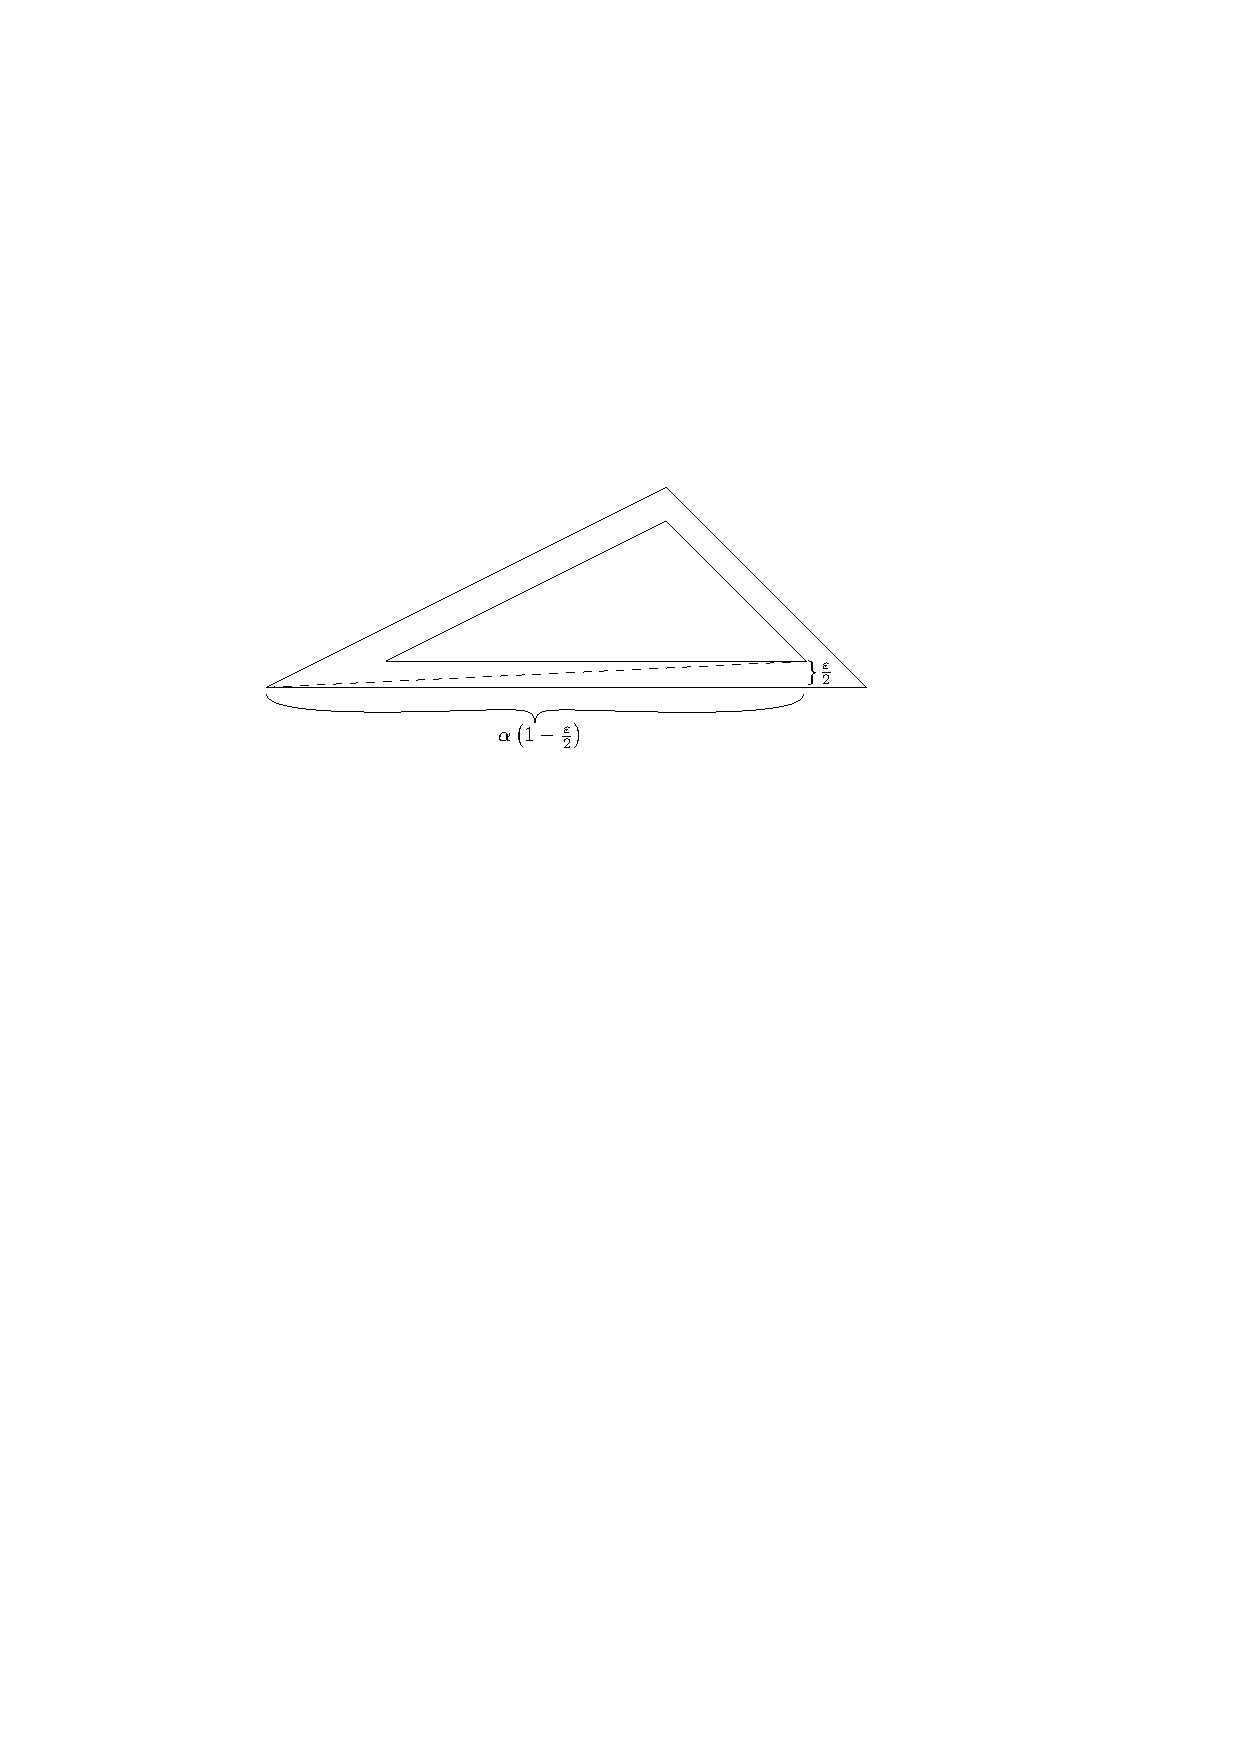
\includegraphics[width=0.6\linewidth]{figs/triangle_shadow}
    \figlab{triangle_with_shadow}
\end{figure}


\subsection{Fat convex regions}

Let $C$ be a convex shape, let $d_+$ be the smallest disk containing
$C$, and $d_-$ be the largest disk contained in $C$. We say that $C$
is $\alpha$-fat if the ratio $\frac{radius(d_+)}{radius(d_-)}$ is at
most $\alpha$. Let $\LL$ be the set of all $\alpha$-fat convex
shapes. In the following, we construct $(\LL, \eps)$-local
$t$-spanners for $t>1$.

We start by proving a structural lemma which will be later used in the
correctness proof.

\begin{claim}
    Let $C$ be an $\alpha$-fat convex shape, and let $C_{1-\eps}$ be
    the $\epsilon$ core of $C$. The shortest segment $\overline{pq}$
    such that $p,q\in\partial C$ and
    $\overline{pq}\cap C_{1-\eps}\neq \emptyset$ is of length at
    least %TO DO.
\end{claim}

\begin{proof}
    Let $d_-$ and $d_+$ be two disks, such that
    $d_-\subseteq C\subseteq d_+$, and
    $\frac{radius(d_+)}{radius(d_-)}=\alpha$, and let $\overline{pq}$
    be the a shortest segment. We assume
    $\overline{pq} \cap C_{1-\eps}$ is a single point $s$.
\end{proof}


\bibliographystyle{alpha}
% \bibliography{shortcuts,geometry}
\bibliography{ft_spanner}

\end{document}
